In this chapter, we provide information on the evaluation of the experiments described in the previous chapters. Below, we indicate which data set is used, how it is partitioned, which models are used, among other details. In the end, we provide an overview of all of the executed experiments, compared to the literature.

\section{Data Set}

The data set used for the experiments is the MNIST\cite{lecun2010mnist} data set. The MNIST data set includes 70 000 images of handwritten digits from 0 to 9, where each image is 28 by 28 pixels. Some samples can be visualized in \autoref{fig:mnist}.

\begin{figure}[!htp]
    \centering
    \centering
    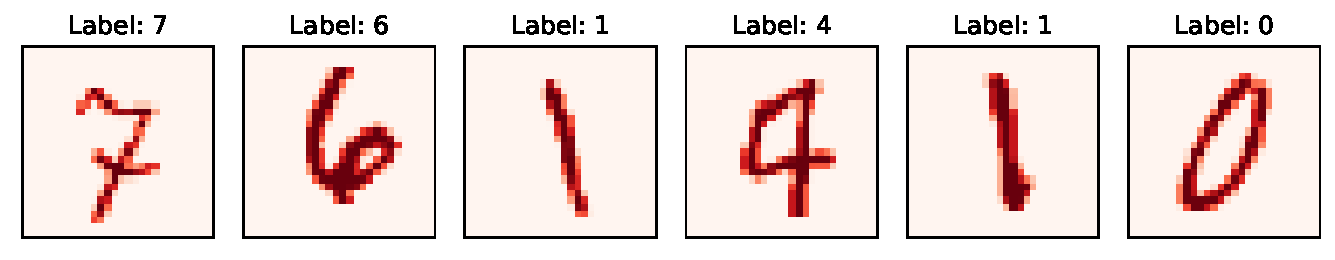
\includegraphics[width=1\textwidth]{graphics/mnist.pdf}
    \caption{MNIST Example Samples}
    \label{fig:mnist}
\end{figure}

Not only is it a widely known data set, but also used by the majority of the reviewed works, as can be seen in \autoref{tab:data_distribution}. Since we will compare our accuracy with the original works in order to validate our results, we need to ensure that the configurations are as similar as possible.

\section{Data Partitioning}

In this section, we show the horizontal and vertical data partitioning according to the methods described in \Cref{chapter:methodology}. To divide the data horizontally, we used a publicly available tool\footnote{\url{https://github.com/TsingZ0/PFL-Non-IID}} that supports partitioning the MNIST dataset directly using the Dirichlet distribution. We did so for 5, 10, 25 and 50 clients.

On \autoref{fig:horizontal_dist}, you can visualize the \textit{non-iid} horizontal partitioning for 10 clients. It is possible to see how \textit{non-iid} the distribution is, both in terms of samples amount and in terms of class distribution. For example, client 7 has many samples from classes 2 and 4, while having none of the remaining classes. At the same time, client 10 has a few samples from classes 0, 1, 2 and 9 and many from class 7.

\begin{figure}[!ht]
    \centering
    \centering
    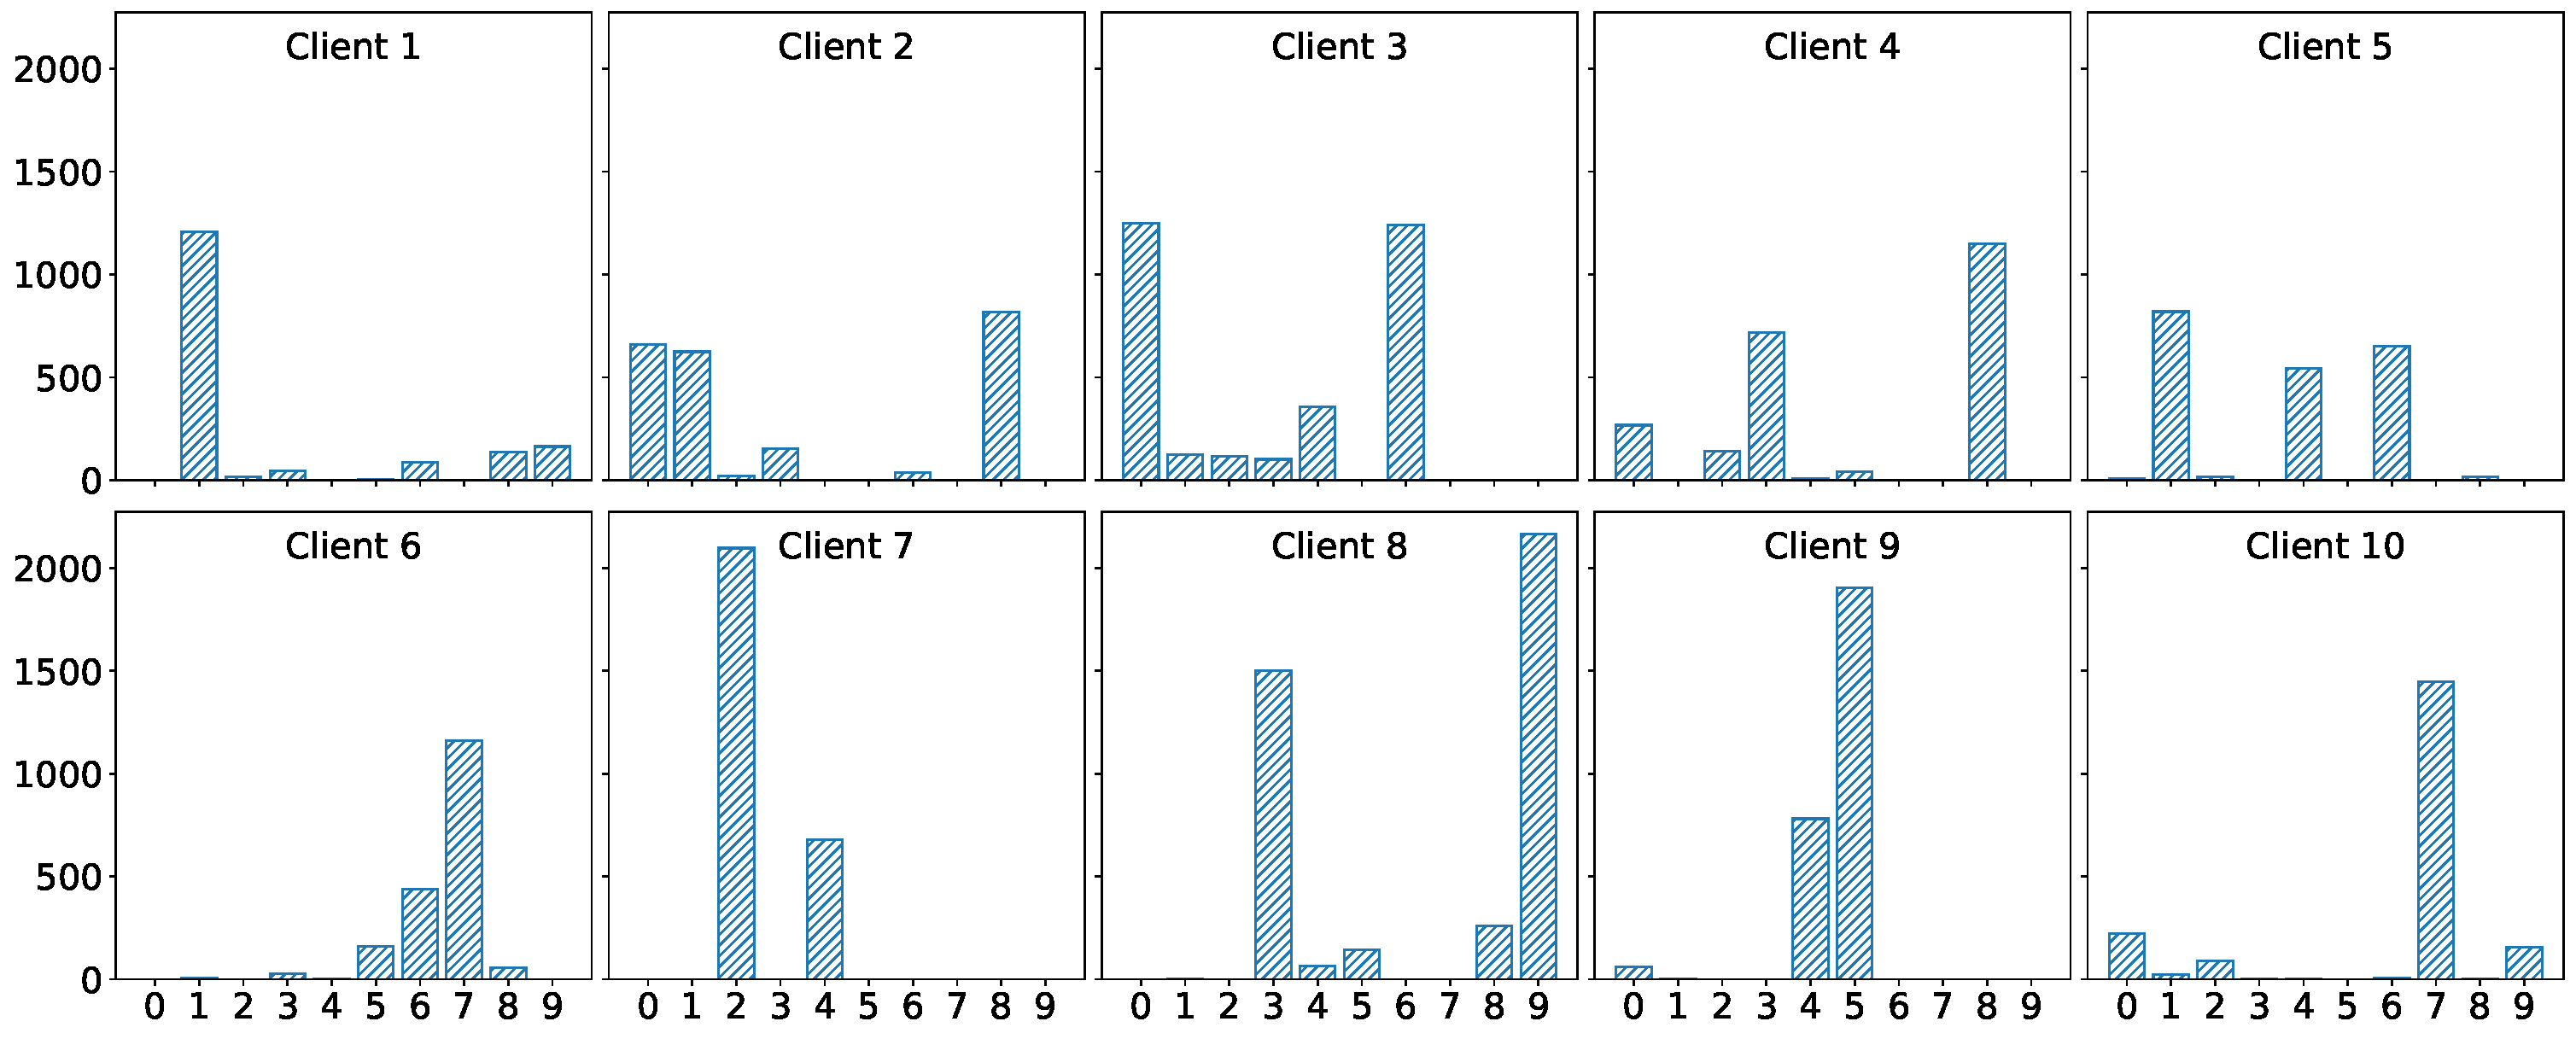
\includegraphics[width=1\textwidth]{graphics/10_dist.pdf}
    \caption{Horizontal Data Distribution For 10 Clients}
    \label{fig:horizontal_dist}
\end{figure}

Regarding vertically partitioning data, it was mentioned in \Cref{subsection:verticalpartitioning} that more details would be provided in the present chapter. The vertical data partitioning highly depends on both the model and the data set. For this experiment, we will use a Split-CNN which will be introduced in the next section. To use such model, the owner is expected to have the labels, while the clients are expected to some features of each sample. In the case of the MNIST dataset, we can think of the features as vertical segments of the image. To divide a 28 by 28 image sample between 2 clients, for example, we split the image into two 14 by 28 segments, as depicted in \autoref{fig:vertical_dist}.

\begin{figure}[!ht]
    \centering
    \centering
    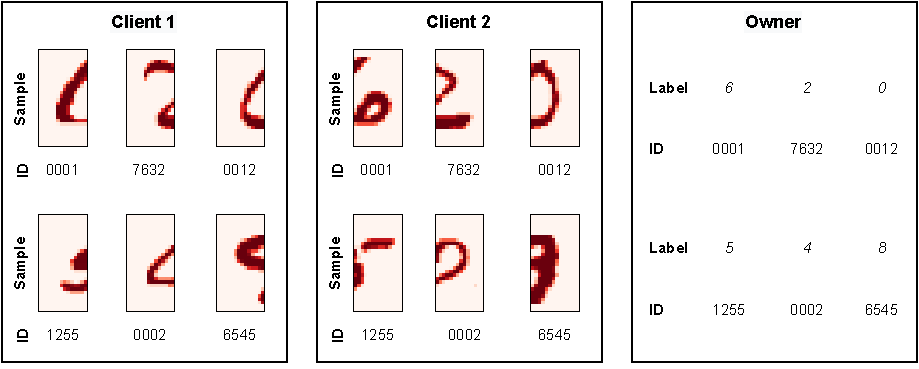
\includegraphics[width=1\textwidth]{graphics/vertical_partitioning.pdf}
    \caption{Vertical Data Distribution for 2 Clients}
    \label{fig:vertical_dist}
\end{figure}

\section{Machine Learning Models}

The models used on this work are simple models based on previous literature. The goal of this work is not to provide the most efficient, or accurate, model. Therefore, we do not dive into the details of the models. The models used for horizontal and vertical training are succinctly explained below.

For horizontal training, we use a simple Convolutional Neural Network (CNN) with three levels of convolution intercalated with max pooling to reduce overfitting. These layers are followed by a flattening layer and two dense layers that culminate in the output. The layer details can be seen in \autoref{tab:cnn}.

\begin{table}[!h]
    \begin{tabular}{c|c}
        \hline \hline
        Layer Type       & Output Shape \\ \hline \hline
        Convolutional 2D & (26, 26, 32) \\ \hline
        Max Pooling 2D   & (13, 13, 32) \\ \hline
        Convolutional 2D & (11, 11, 64) \\ \hline
        Max Pooling 2D   & (5, 5, 64)   \\ \hline
        Convolutional 2D & (3, 3, 64)   \\ \hline
        Flatten          & (576)        \\ \hline
        Dense            & (64)         \\ \hline
        Dense            & (10)         \\ \hline
    \end{tabular}
    \caption{CNN Model}
    \label{tab:cnn}
\end{table}

For vertical training, we use a dual-headed, or four-headed, Split-CNN \cite{10.1145/3297858.3304038, 10.48550/arxiv.2104.00489}, depending on whether we have two, or four, clients. The model at the clients is the head model, while the model at the servers is the tail model. To train this model, each client gives their input data to the models and collects the output of the last layer. Then, this intermediate output is sent to the servers, which are then given to the tail model. The servers calculate the gradients, which are then backpropagated to the clients. For more details, please consult the original works where the workings of this model are given in more detail. On \autoref{tab:splitnn} you can see the details of the dual-headed Split-CNN model.

\begin{table}[!h]
    \begin{subtable}[h]{0.49\textwidth}
        \centering
        \begin{tabular}{c|c}
            \hline \hline
            Layer Type       & Output Shape \\ \hline \hline
            Convolutional 2D & (26, 12, 32) \\ \hline
            Max Pooling 2D   & (13, 6, 32) \\ \hline
            Convolutional 2D & (11, 11, 64) \\ \hline
            Max Pooling 2D   & (5, 2, 64)   \\ \hline
        \end{tabular}
        \caption{Head}
    \end{subtable}
    \hfill
    \begin{subtable}[h]{0.49\textwidth}
        \centering
        \begin{tabular}{c|c}
            \hline\hline
            Layer Type     & Output Shape \\ \hline\hline
            2 Input Layers & (5, 2, 64)   \\ \hline
            Concatenation  & (5, 2, 128)  \\ \hline
            Flatten        & (1280)       \\ \hline
            Dense          & (512)        \\ \hline
            Dense          & (256)        \\ \hline
            Dense          & (10)         \\ \hline
        \end{tabular}
        \caption{Tail}
     \end{subtable}
     \caption{Split-CNN Dual-Headed Model}
     \label{tab:splitnn}
\end{table}

\section{Hardware and Software Specifications}

The experiments were executed in a remote machine whose hardware and software specifications can be found in \autoref{tab:temps}. Due to resource limitations, it was not possible to have a machine with GPU. Furthermore, if we consider that Federated Learning systems are being run in IoT clients, it is unlikely that such low-powered devices would have a GPU available. In addition, the MNIST dataset and the models in use are relatively simple, which means that they can be easily trained using a CPU. Nonetheless, it is worth mentioning that the training process would be faster in machines with a GPU.

\begin{table}[!h]
    \begin{subtable}[h]{0.59\textwidth}
        \centering
        \begin{tabular}{l|l} \hline \hline
            Hardware & Model                                    \\ \hline \hline
            CPU      & AMD Ryzen 5 3600 6-Core 4.2 GHz          \\ \hline
            RAM      & 64 GB                                    \\ \hline
            Disk     & 500 GB NVMe                              \\ \hline
        \end{tabular}
        \caption{Hardware}
        \label{evaluation:hardware}
    \end{subtable}
    \hfill
    \begin{subtable}[h]{0.39\textwidth}
        \centering
        \begin{tabular}{l|l} \hline \hline
            Software            & Version               \\ \hline \hline
            Docker              & 20.10.15              \\ \hline
            Docker Compose      & 2.5.0                 \\ \hline
            Python              & 3.8.13               \\ \hline
            Node.js             & 16.15.0               \\ \hline
            Truffle             & 5.5.13               \\ \hline
            Ganache             & 7.1.0               \\ \hline
            Solidity            & 0.5.16               \\ \hline
        \end{tabular}
        \caption{Software}
        \label{evaluation:software}
     \end{subtable}
     \caption{Hardware and Software Specifications}
     \label{tab:temps}
\end{table}

\section{Results}

\autoref{tab:experiments} presents a summary of all of our experiments, as well as other works. On it, it is possible to see the configuration of all of the experiments that were executed. Due to space limitations, not all information is presented on the table. All experiments use the MNIST data set, except for the works \cite{10.48550/arxiv.2007.03856, 10.48550/arxiv.2011.07516} whose data set is unknown. In addition, all the experiments were executed with 50 rounds, except for \cite{9170559} which is also unknown. We can see that our results, in terms of accuracy, are within the range of the original works of the scoring algorithms. Therefore, we can validate our results.

The detailed analysis of the results of each experiment are presented in the following chapters. \Cref{chapter:analysis:consensus_algorithms} presents the analysis on the consensus algorithms experiments. \Cref{fig:participations_client} analyzes the results on the participant selection techniques experiments. \Cref{chapter:analysis:scoring} presents the analysis on the scoring techniques experiments. \Cref{chapter:analysis:clients} analyzes the results on the impact of the number of training clients. \Cref{chapter:analysis:privacy} presents the results and analysis of the impact of different privacy degrees. Finally, \Cref{chapter:vertical} presents the results of the Proof of Concept of Vertical Federated Learning applied in a Blockchain-based Federated Learning environment.

\begin{landscape}

\begin{table}[]
\begin{tabular}{c|c|c|c|c|c|c|c|c|c|c} \hline \hline
\multirow{2}{*}{Group}                                                                      & \multirow{2}{*}{ID} & \multirow{2}{*}{Work}                     & Consensus                  & \multirow{2}{*}{Clients} & Participants            & Scoring                        & \multicolumn{2}{c}{Data}                & Privacy                & \multirow{2}{*}{Accuracy}              \\ 
                                                                                            &                     &                                            & Algorithms                 &                          & Selection     &                       & P          & D       & Degree                 &                                        \\ \hline \hline
\multirow{3}{*}{\begin{tabular}[c]{@{}c@{}}Consensus\\ Algorithms\end{tabular}}             & 1                   & \multirow{3}{*}{$\star$}                         & PoA                        & \multirow{3}{*}{25}      & \multirow{3}{*}{Random} & \multirow{3}{*}{None}          & \multirow{3}{*}{H} & \multirow{3}{*}{N} & \multirow{3}{*}{None}  & 98.54                                  \\ \cline{2-2}\cline{4-4}\cline{11-11}
                                                                                            & 2                   &                                            & PoW                        &                          &                         &                                &                    &                    &                        & 98.35                                  \\ \cline{2-2}\cline{4-4}\cline{11-11}
                                                                                            & 3                   &                                            & IBFT                       &                          &                         &                                &                    &                    &                        & 98.90                                  \\\hline
\multirow{2}{*}{\begin{tabular}[c]{@{}c@{}}Participant Selection\\ Techniques\end{tabular}} & 1                   & \multirow{2}{*}{$\star$}                         & \multirow{2}{*}{PoA}       & \multirow{2}{*}{25}      & Random                  & \multirow{2}{*}{None}          & \multirow{2}{*}{H} & \multirow{2}{*}{N} & \multirow{2}{*}{None}  & 98.54                                  \\ \cline{2-2}\cline{6-6}\cline{11-11}
                                                                                            & 4                   &                                            &                            &                          & F.C.F.S &                                &                    &                    &                        & 98.18                                  \\ \hline
\multirow{4}{*}{\begin{tabular}[c]{@{}c@{}}Scoring\\ Techniques\end{tabular}}               & 1                   & \multirow{4}{*}{$\star$}                         & \multirow{4}{*}{PoA}       & \multirow{4}{*}{25}      & \multirow{4}{*}{Random} & None                           & \multirow{4}{*}{H} & \multirow{4}{*}{N} & \multirow{4}{*}{None}  & 98.54                                  \\
                                                                                            & 10                  &                                            &                            &                          &                         & BlockFlow                      &                    &                    &                        & 97.04                                  \\
                                                                                            & 14                  &                                            &                            &                          &                         & Marginal Gain                  &                    &                    &                        & 98.58                                  \\
                                                                                            & 18                  &                                            &                            &                          &                         & Multi-KRUM                     &                    &                    &                        & 97.00                                  \\ \hline
\multirow{21}{*}{\begin{tabular}[c]{@{}c@{}}Number\\ of Clients\end{tabular}}               & 5                   & \multirow{4}{*}{$\star$}                         & \multirow{4}{*}{PoA}       & 5                        & \multirow{4}{*}{Random} & \multirow{4}{*}{None}          & \multirow{4}{*}{H} & \multirow{4}{*}{N} & \multirow{4}{*}{None}  & 97.76                                  \\
                                                                                            & 6                   &                                            &                            & 10                       &                         &                                &                    &                    &                        & 97.06                                  \\
                                                                                            & 1                   &                                            &                            & 25                       &                         &                                &                    &                    &                        & 98.54                                  \\
                                                                                            & 7                   &                                            &                            & 50                       &                         &                                &                    &                    &                        & 98.88                                  \\ \hline
                                                                                            & 8                   & \multirow{4}{*}{$\star$}                         & \multirow{4}{*}{PoA}       & 5                        & \multirow{4}{*}{Random} & \multirow{4}{*}{BlockFlow}     & \multirow{4}{*}{H} & \multirow{4}{*}{N} & \multirow{4}{*}{None}  & 97.94                                  \\
                                                                                            & 9                   &                                            &                            & 10                       &                         &                                &                    &                    &                        & 85.92                                  \\
                                                                                            & 10                  &                                            &                            & 25                       &                         &                                &                    &                    &                        & 97.04                                  \\
                                                                                            & 11                  &                                            &                            & 50                       &                         &                                &                    &                    &                        & 97.84                                  \\ \hline
                                                                                            & \multirow{3}{*}{}   & \multirow{3}{*}{\cite{10.48550/arxiv.2007.03856}} & \multirow{3}{*}{PoW}       & 25                       & \multirow{3}{*}{?}      & \multirow{3}{*}{BlockFlow}     & \multirow{3}{*}{H} & \multirow{3}{*}{?} & \multirow{3}{*}{$\epsilon =$ ?} & \multirow{3}{*}{$\geq$ 85.00} \\
                                                                                            &                     &                                            &                            & 50                       &                         &                                &                    &                    &                        &                                        \\
                                                                                            &                     &                                            &                            & 100                      &                         &                                &                    &                    &                        &                                        \\ \hline
                                                                                            & 12                  & \multirow{4}{*}{$\star$}                         & \multirow{4}{*}{PoA}       & 5                        & \multirow{4}{*}{Random} & \multirow{4}{*}{Marginal Gain} & \multirow{4}{*}{H} & \multirow{4}{*}{N} & \multirow{4}{*}{None}  & 89.12                                  \\
                                                                                            & 13                  &                                            &                            & 10                       &                         &                                &                    &                    &                        & 96.62                                  \\
                                                                                            & 14                  &                                            &                            & 25                       &                         &                                &                    &                    &                        & 98.58                                  \\
                                                                                            & 15                  &                                            &                            & 50                       &                         &                                &                    &                    &                        & 98.90                                  \\ \hline
                                                                                            &                     & \cite{10.48550/arxiv.2011.07516}                  & ?                          & ?                        & ?                       & Marginal Gain                  &                    & ?                  & None                   & $\geq$ 90.00                  \\ \hline
                                                                                            & 16                  & \multirow{4}{*}{$\star$}                         & \multirow{4}{*}{PoA}       & 5                        & \multirow{4}{*}{Random} & \multirow{4}{*}{Multi-KRUM}    & \multirow{4}{*}{H} & \multirow{4}{*}{N} & \multirow{4}{*}{None}  & 96.68                                  \\
                                                                                            & 17                  &                                            &                            & 10                       &                         &                                &                    &                    &                        & 98.44                                  \\
                                                                                            & 18                  &                                            &                            & 25                       &                         &                                &                    &                    &                        & 97.00                                  \\
                                                                                            & 19                  &                                            &                            & 50                       &                         &                                &                    &                    &                        & 98.48                                  \\
                                                                                            &                     & \cite{9170559}                                    & PoS, pBFT                  &                          & ?                       &                                &                    & I                  & $\epsilon =$ 10                 & 98.00                                  \\
\multirow{18}{*}{\begin{tabular}[c]{@{}c@{}}Privacy\\ Degrees\end{tabular}}                 & 1                   & \multirow{3}{*}{$\star$}                         & \multirow{3}{*}{PoA}       & \multirow{3}{*}{25}      & \multirow{3}{*}{Random} & \multirow{3}{*}{None}          & \multirow{3}{*}{H} & \multirow{3}{*}{N} & None                   & 98.54                                  \\
                                                                                            & 19                  &                                            &                            &                          &                         &                                &                    &                    & $\epsilon =$ 5                  & 98.18                                  \\
                                                                                            & 20                  &                                            &                            &                          &                         &                                &                    &                    & $\epsilon =$ 1                  & 80.22                                  \\
                                                                                            & 10                  & \multirow{3}{*}{$\star$}                         & \multirow{3}{*}{PoA}       & \multirow{3}{*}{25}      & \multirow{3}{*}{Random} & \multirow{3}{*}{BlockFlow}     & \multirow{3}{*}{H} & \multirow{3}{*}{N} & None                   & 97.04                                  \\
                                                                                            & 21                  &                                            &                            &                          &                         &                                &                    &                    & $\epsilon =$ 5                  & 94.00                                  \\
                                                                                            & 22                  &                                            &                            &                          &                         &                                &                    &                    & $\epsilon =$ 1                  & 84.68                                  \\
                                                                                            &                     & \cite{10.48550/arxiv.2007.03856}                  & PoW                        & 25                       & ?                       & BlockFlow                      & H                  & ?                  & $\epsilon =$ ?                  & $\geq$ 85.00                  \\
                                                                                            & 14                  & \multirow{3}{*}{$\star$}                         & \multirow{3}{*}{PoA}       & \multirow{3}{*}{25}      & \multirow{3}{*}{Random} & \multirow{3}{*}{Marginal Gain} & \multirow{3}{*}{H} & \multirow{3}{*}{N} & None                   & 98.58                                  \\
                                                                                            & 23                  &                                            &                            &                          &                         &                                &                    &                    & $\epsilon =$ 5                  & 98.36                                  \\
                                                                                            & 24                  &                                            &                            &                          &                         &                                &                    &                    & $\epsilon =$ 1                  & 92.26                                  \\
                                                                                            &                     & \cite{10.48550/arxiv.2011.07516}                  & ?                          & ?                        & ?                       & Marginal Gain                  &                    & ?                  & None                   & $\geq$ 90.00                  \\
                                                                                            & 18                  & \multirow{3}{*}{$\star$}                         & \multirow{3}{*}{PoA}       & \multirow{3}{*}{25}      & \multirow{3}{*}{Random} & \multirow{3}{*}{Multi-KRUM}    & \multirow{3}{*}{H} & \multirow{3}{*}{N} & None                   & 97.00                                  \\
                                                                                            & 25                  &                                            &                            &                          &                         &                                &                    &                    & $\epsilon =$ 5                  & 94.70                                  \\
                                                                                            & 26                  &                                            &                            &                          &                         &                                &                    &                    & $\epsilon =$ 1                  & 91.00                                  \\
                                                                                            &                     & \cite{Peyvandi2022}                               & ?                          & \multirow{4}{*}{?}       & Random                  & \multirow{4}{*}{Multi-KRUM}    &                    & N                  & $\epsilon =$ ?                  & 94.39                                  \\
                                                                                            &                     & \multirow{3}{*}{9170559}                   & \multirow{3}{*}{PoS, pBFT} &                          & \multirow{3}{*}{?}      &                                & \multirow{3}{*}{}  & \multirow{3}{*}{I} & $\epsilon =$ 10                 & 98.00                                  \\
                                                                                            &                     &                                            &                            &                          &                         &                                &                    &                    & $\epsilon =$ 5                  & 96.50                                  \\
                                                                                            &                     &                                            &                            &                          &                         &                                &                    &                    & $\epsilon =$ 1                  & 86.00                                  \\
\multirow{2}{*}{\begin{tabular}[c]{@{}c@{}}Vertical Federated\\ Learning\end{tabular}}      & 27                  & \multirow{2}{*}{$\star$}                         & \multirow{2}{*}{PoA}       & 2                        & \multirow{2}{*}{N/A}    & \multirow{2}{*}{N/A}           & \multirow{2}{*}{V} & \multirow{2}{*}{N} & \multirow{2}{*}{None}  &                                        \\
                                                                                            & 28                  &                                            &                            & 4                        &                         &                                &                    &                    &                        &                                       
\end{tabular}
\end{table}

\end{landscape}